\graphicspath{{images/}}

\section{Introduction}
\label{sec:introduction}

The bacterium \textit{Eschericia coli} and yeast \textit{Saccharomyces
  cerevisiae} are unicellular organisms studied as a model prokaryote
and eukaryote respectively.
% Compared to other species bacteria and yeasts have small compact genomes.
Much of their genomes have been conserved in other species over
billions of years of evolution
\citep{OBrien2005inparanoid}. \textit{S.~cerevisiae} was the first
eukaryote to have its entire genome sequenced \citep{goffeau1996life}
and is particularly useful as a model of other eukaryotes such as
human cells. Bacteria and yeasts grow in colonies. In favourable
conditions, growth is exponential and this makes growth rate a major
component of fitness; colonies of faster growing strains quickly come
to dominate populations. At a certain point growth becomes limited and
a stationary phase is reached so pressure also exists to use resources
efficiently. In short, fitness, to a large degree, is governed by
competing pressures on growth rate and yield
\citep{dethlefsen2007performance}. The growth of microbial organisms
can be observed and used to determine fitness estimates
(see~e.g.~\citet{Baryshnikova2010,Addinall2011}). In growth
experiments, cell cultures are commonly grown in one of two types of
medium: on the surface of a nutrient rich solid agar or in a liquid
mixture containing nutrients. In both cases cultures are incubated and
cell density is measured over time. Identical strains can grow
differently in these environments and disagreement in fitness
estimates has been observed \citep{Baryshnikova2010}. Here, I focus on
estimating the fitness of microbes growing on solid agar surfaces.

% The bacterium \textit{Eschericia coli} and yeast \textit{Saccharomyces
%   cerevisiae} are unicellular organisms studied as a model prokaryote
% and eukaryote respectively.
% Bacteria and yeasts grow in
% colonies. In favourable conditions, growth is exponential and this
% makes growth rate a major component of fitness; colonies of faster
% growing strains quickly come to dominate populations. At a certain
% point growth becomes limited and a stationary phase is reached. In
% short, fitness is governed by competing pressures on fast growth rate
% and yield \citep{dethlefsen2007performance}.
% Compared to other species bacteria and yeasts have small compact
% genomes. Many genes have been conserved in other species over billions
% of years of evolution
% \citep{OBrien2005inparanoid}. \textit{S.~cerevisiae} was the first
% eukaryote to have its entire genome sequenced \citep{goffeau1996life}
% and is particularly useful as a model of other eukaryotes such as
% human cells.

% The growth rate of microbial organisms is measurable and is often used
% to determine fitness (see~e.g.~\citet{Addinall2011}). In growth
% experiments, cell cultures are commonly grown in one of two types of
% medium: on the surface of a nutrient rich solid agar or in a liquid
% mixture containing nutrients. In both cases cultures are incubated and
% cell density is measured over time. Identical strains can grow
% differently in these environments and disagreement in fitness
% estimates has been observed \citet{Baryshnikova2010}. Here, I focus on
% estimating the fitness of microbes growing on solid agar surfaces.

%%% Genetic interaction, SGA and QFA %%%

Fitness estimates can be used to infer genetic interaction or drug
response and high-throughput methods allow this to be conducted on a
genome-wide scale (see e.g. \citet{Costanzo2010,Andrew2013}). In a
typical genetic interaction screen a strain is made with a background
mutation in a query gene. Double mutants are created by introducing a
second deletion to this strain. By comparing the growth of double
mutants with controls containing a neutral background mutation
(effectively single mutants), genetic interactions can be inferred. If
a strain is fitter than predicted given the observation of control
fitness, then the deletion is said to suppress the defect of the query
mutation. If a strain is less fit than predicted given the observation
of control fitness, then the deletion is said to enhance the defect of
the query mutation. Either scenario suggests that the two genes
interact. Due to redundancy, single deletions are often
non-lethal. This allowed \citet{Costanzo2010} to explore genetic
interactions for \(\sim\)75\% of the \textit{S. cerevisiae} genome.


Synthetic Genetic Array (SGA) and Quantitative Fitness Analysis (QFA)
are high-throughput methods for obtaining quantitative fitness
estimates for microbial cultures grown on solid agar
\citep{Baryshnikova2010sga,Banks2012}. Typically 100s or 1000s of
deletions with a common background mutation are pinned or inoculated
in a rectangular array on a solid agar plate. Many plates with
different query genes and deletions are grown in high-throughput to
explore whole genomes. I study data from QFA, which includes
quantitative estimation of fitness by measurement and fitting of
growth curves. In a typical QFA procedure, liquid cultures are
incolulated onto solid agar in a 16x24 rectangular array of 384
spots. Inoculum density can be varied to capture more or less of the
growth curve and the most dilute cultures are inoculated with
\(\sim\)100 starting cells \citep{Addinall2011}. Plates are grown in a
temperature controlled incubator and removed to be photographed
periodically throughout the growth curve. Photographs are of whole
plates and growth typically covers several days to capture both the
exponential and stationary growth phases. Colonyzer
\citep{Lawless2010} processes optical density measurements in
photographs to produce a timecourse of cell density estimates for each
culture. In past analysis, the logistic growth model was independently
fit to the timecourse of each culture and fitness estimates were
defined in terms of parameters of this model, namely the growth
constant \(r\) and carrying capacity \(K\). In contrast, SGA typically
uses a larger array of 1536 pinned cultures and a single endpoint
assay of culture area to quantify growth. The differential form and
solution of the logistic model \citep{Verhulst1845} are given in
(\ref{eq:logistic_model}), where \(C\) represents cell density and
\(C(0)\) is cell density at time zero.
% Logistic model equations
\begin{subequations}
  \label{eq:logistic_model}
  \begin{align}
    &\dot{C} = rC\left(1 - \frac{C}{K}\right)\\
    &C(t) = \frac{KC(0)e^{rt}}{K + C(0)(e^{rt}-1)}
  \end{align}
\end{subequations}
%
The logistic model is a simple mechanistic model describing
self-limiting growth and has a sigmoidal solution. Growth begins
exponentially with rate \(rC\) and curtails as the population size
increases and cells begin to compete for some limited resource. Cell
density reaches a final carrying capacity \(K\) at the stationary
phase. In QFA, nutrients must diffuse through agar to reach cells
growing on the surface. It is plausible that the carrying capacity
\(K\) represents the point at which nutrients either run out or growth
becomes limited by the diffusion of nutrients and is approximately
stationary. Fitting the logistic model to QFA data requires plate
level or culture level parameters for \(C(0)\) and culture level
parameters for \(r\) and \(K\) making 769 or 1152 parameters per 384
culture plate.

The growth constant \(r\) could be used as a fitness measure. However,
\citet{Addinall2011} define a more complicated fitness measure as the
product of Maximum Doubling Rate (MDR) and Maximum Doubling Potential
(MDP) which they calculate from logistic model parameters. MDR measures
the doubling rate at the beginning of the exponential growth phase,
when growth is fastest, and MDP is the number of divisions which a
culture undergoes from inoculation to the stationary phase.
%
\begin{subequations}
  \label{eq:MDR_MDP}
    \begin{align}
      MDR &= \frac{r}{log\left(\frac{2(K-C(0))}{K-2C(0)}\right)}\\
      MDP &= \frac{log\left(\frac{K}{C(0)}\right)}{log(2)}
    \end{align}
\end{subequations}
%
To improve the quality of fits, QFA now uses the generalised logistic
model which requires an extra shape parameter for each culture
\citep{Banks2012}. Standard and generalised logistic model \(r\) are
not equivalent so comparison relies on MDR and MDP as fitness
measures. The analysis of QFA data using both models is available
through the QFA R package \citep{qfa2016}.

%%%% up to here

% //Could remove//\citet{Addinall2011} used QFA and
% \textit{S. cerevisiae} to screen for genes involved in telomere
% stability which is related to ageing and cancer and has implications
% for human health and disease. Hits from this study have been
% successfully followed to discover new biology
% \citep{Holstein20141259}. (To be honest I have no idea about the
% significance of what they found in this paper. We had a more general
% focus. If I have room I should probably try and sell the potential
% benefits and past successes of QFA a bit more to expand the
% motivation. Obviously I will mention the Addinall paper when I
% describe p15 in the methods.)  //Could remove//
% Example use of QFA by Addinall \citep{Addinall2011} telomeres.
% And follow up Holstein and Clark \citep{Holstein20141259}

Since QFA aims to determine differences in the fitness of microbial
strains from measurements of differences in growth, fast and slow
growing cultures are often grown
side-by-side. Figure~\ref{fig:p15_section} shows a section of a QFA
plate from a study by \citet{Addinall2011} where this is the
case. Cultures were inoculated with approximately equal cell density
but have grown at different rates and to visibly different sizes after
\(\sim\)2.5 days. Despite starting with the same amount of nutrients
and growing at different rates, there is a characteristic timescale
for the cessation of growth. This suggests a global growth-limiting
effect, which I believe to be caused by an interaction between
cultures. I test the hypothesis that the interaction is a competition
effect due to the diffusion of nutrients along gradients formed
between fast and slow growing neighbours. This has implications for
growth estimates; competition will cause growth to appear faster or
slower for each neighbour than would be observed if they grew
independently. The experiment shown in Figure~\ref{fig:stripes_images}
provides further support for a nutrient competition effect. The same
cultures were grown in alternate columns on two separate plates but
with cultures added or removed from the neighbouring columns
inbetween. Cultures in Figure~\ref{fig:stripes_images}a, where
neighbours were removed, grew larger
%(how much? I can look at the data myself) **
than the same cultures in Figure~\ref{fig:stripes_images}b, where
neighbours were added. This suggests that an interaction between
neighbours is present and may be affecting fitness estimates. Current
QFA analysis using the logistic model assumes that cultures grow
independently and ignores possible competition effects between
neighbours. The sigmoidal curve of the logistic model poorly fits QFA
data in many cases
%% evidence? **
and this may be due to competition effects. I aim to fit a network
model of nutrient dependent growth and diffusion to QFA data to try to
correct for competition, to increase the accuracy and precision of
fitness estimates, and to improve the fit of individual growth curves.

\begin{Figure}
  \centering
  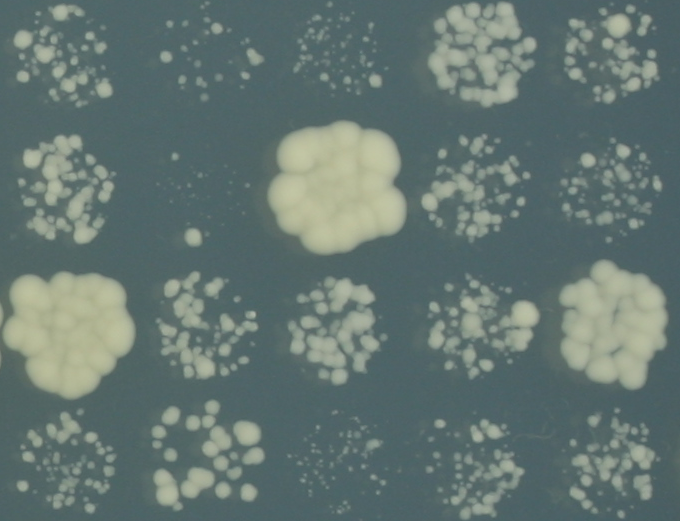
\includegraphics[width=\linewidth]{p15_section/p15_section_4x5_5_18}
  \captionof{figure}{\textbf{4x5 section of a QFA plate (P15).}
    Cropped from a 16x24 format solid agar plate inoculated with
    dilute \textit{S. cerevisiae} cultures. Image captured at
    \(\sim\)2.5d after inoculation and incubation at 27\(^{\circ}C\).}
  \label{fig:p15_section}
\end{Figure}
\begin{Figure}
  \centering
  \includegraphics[width=\linewidth]{stripes/final/striped}
  \includegraphics[width=\linewidth]{stripes/final/filled}
  \captionof{figure}{\textbf{A QFA experiment designed to examine
      competition.}  A) ``Stripes'' QFA plate inocluated with a more
    concentrated \textit{S. Cerevisiae} inoculum (no cells inocluated
    on alternate columns). B) ``Filled'' plate: Same as in A, but with
    strains of similar growth rate inoculated in the positions missing
    in A.}
  \label{fig:stripes_images}
\end{Figure}

Competition effects could be dealt with experimentally by randomising
the location of cultures on repeated plates. This does not require
explicit knowledge or modelling of the source of interaction but
reduces throughput, so, if possible, a modelling approach is
desirable. Poisoning of cultures by a signal molecule such as ethanol,
which \textit{S. cerevisiae} produces in the metabolism of sugars by
fermentation, is another possible source of interaction.
%%%% Quorum Sensing %%%%
QFA does not measure nutrients or signal, so if more than one source
of interaction exists, it becomes very difficult to fit a model and
randomisation may be the best approach. QFA data for edge cultures is
noisy due to reflections from plate edges. This is only partially
corrected for by Colonyzer \citep{Lawless2010} and, as a result, data
for edge cultures is usually discarded. \citet{Addinall2011} grow
repeats of a neutral deletion in edge locations, rather than leaving
them empty, because of concerns about competition. In an SGA study,
\citet{Baryshnikova2010} use statistical techniques to correct for
competition between fast and slow growing neighbours in end-point
assays of culture area. I expect that modelling competition for
nutrients explicitly will provide a better correction using fewer
repeats. QFA uses more information than SGA by fitting whole growth
curves, rather than a single endpoint assay, so a modelling approach
also promises to be more powerful. Furthermore, modelling may identify
and explain the source of competition. Simulations from an accurate
model will allow assessment of alternative of experimental designs and
prediction of ways to reduce competition effects.

% Could also talk about ethanol and quorum sensing and amonia when I get
% to competition.


% //Diffusion Equation: I am probably going to have to repeat this
% when I get to the discussion so I could just leave until then.//
% Previous model of nutrient diffusion.
\citet{Reo2014} use a diffusion equation model to simulate nutrient
dependent growth of a single bacterial culture on a pertri dish in
two-dimensions. They create a sink for nutrients from culture growth
and equate the flux of nutrients through culture area with the rate of
increase in culture size. They model culture area as varying and keep
culture density constant. This model could be adapted for QFA by
approximating culture area as constant and allowing culture density to
vary. However, it would be too computationally intensive to fit a
similar model to a full QFA plate in three-dimensions, especially if
the model is to be used to process many plates from high-throughput
experiments. Therefore, a simpler model of nutrient diffusion is
required.
%//Diffusion Equation//

Lawless proposed a model of nutrient dependent growth and
competition (\ref{eq:reaction},\ref{eq:competition_model}),
hereinafter the competition model, using mass action kinetics and
network diffusion (Figure~\ref{fig:comp_model_schematic}). He
represents the nutrient dependent division of cells with the reaction
equation,
\begin{equation}
  \label{eq:reaction}
    C + N \xrightarrow[]{b} 2C,
\end{equation}
where \(C\) is a cell, \(N\) is the amount of nutrient required for
one cell division, and \(b\) is a rate constant for the reaction. (The
identity of the limiting nutrient \(N\) is unknown but possible
candidates are sugar and nitrogen.) He defines separate reactions
(\ref{eq:reaction}) with growth constant \(b_{i}\) for each culture,
indexed \(i\), on a plate and uses mass action kinetics to derive rate
equations for the amount of cells and nutrients associated with each
culture, \(C_{i}\) and \(N_{i}\). This gives the rate equation for
\(C_{i}\) (\ref{eq:competition_model}a) and the first term in the rate
equation for \(N_{i}\) (\ref{eq:competition_model}b).

\begin{subequations}
  \label{eq:competition_model}
  \begin{align}
         % \frac{dC_{i}}{dt}& = b_{i}N_{i}C_{i},\\
         % \frac{dN_{i}}{dt}& = - b_{i}N_{i}C_{i} - k\sum_{j \epsilon \delta_i}(N_{i} - N_{j}).
         \dot{C_{i}}& = b_{i}N_{i}C_{i},\\
         \dot{N_{i}}& = - b_{i}N_{i}C_{i} - k\sum_{j \epsilon \delta_i}(N_{i} - N_{j}).
  \end{align}
      % \right\ Hello
      % \qquad
\end{subequations}


To arrive at the full competition model, he models the diffusion of
nutrients along gradients between a culture \(i\) and its closest
neighbours \(\delta_{i}\) by the second term in
(\ref{eq:competition_model}b), where \(k\) is a nutrient diffusion
constant. This can also be expressed as a series of reversible
first-order reactions of the form
\begin{equation}
  \label{eq:diffusion_reaction}
  \left.\begin{aligned}
  &N_{i} \xrightarrow[]{k} N_{j}\\
  &N_{j} \xrightarrow[]{k} N_{i}
       \end{aligned}
 \right.
 \qquad \forall~j \in \delta_{i},
  % \begin{align}
  % \end{align}
\end{equation}
% \begin{equation}
%   \label{eq:diffusion_reaction}
%   \left.
%     N_{i} \xrightleftarrow[k]{k} N_{j}\\
%  \right.\qquad
%     \forall~j \in \delta_{i},
%   % \begin{align}
%   % \end{align}
% \end{equation}
and modelled with mass action kinetics. Unlike the logistic
model~(\ref{eq:logistic_model}), the competition model has no
analytical solution, and must instead be solved numerically. If \(k\)
is set to zero, the competition model reduces to the mass action
equivalent of the logistic model, hereinafter the mass-action logistic
model, and has the same sigmoidal solution. In this limit, parameters
of the competition model can be converted in terms of parameters the
logistic model (see Section~\ref{sec:parameter_conversion}).
%%%% could go to methods %%%%
When the competition model is fit to QFA data, \(C_{i}\) is observed
and \(N_{i}\) is hidden. Inoculum density, \(C(0)\), is often below
detectable levels. By assuming that incolulum density is the same for
all cultures and that nutrients are distributed evenly throughout the
agar at time zero, initial values of cells and nutrients, \(C(0)\) and
\(N(0)\), can be inferred at the plate level. \(k\) is assumed to be
constant across the plate but must be inferred. There is a growth
constant, \(b_{i}\), for each of 384 cultures on a typical QFA plate
making 387 parameters in total. The competition model shares more
information between cultures and has less than half the number of
parameters of either the standard or generalised logistic model
\citep{Banks2012,qfa2016}.
%%%%%%%%%%%%%%%%%%%%%%%%%%%%%%%
\begin{Figure}
  \centering
  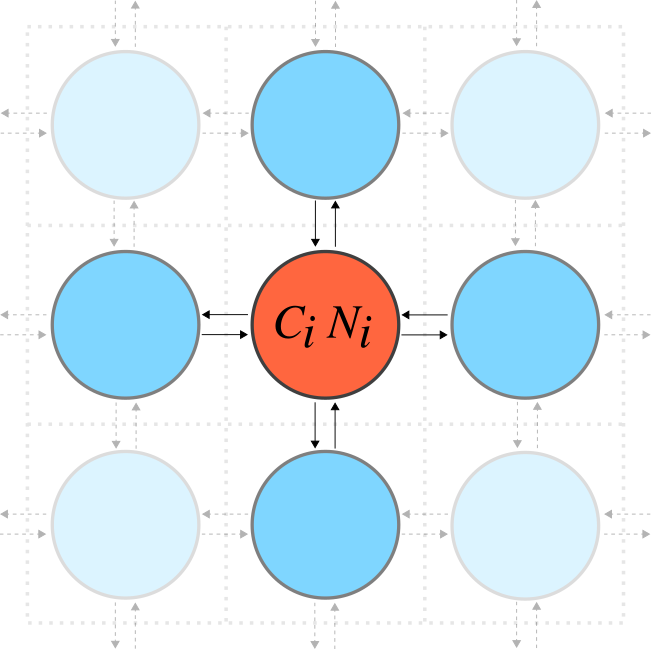
\includegraphics[width=\linewidth]{comp_model/comp_model_schematic2}
  \captionof{figure}{\textbf{Schematic of the competition model.}
    Each circle represents a culture, indexed \(i\), growing in a
    rectangular array on the surface of solid agar containing
    nutrients. Arrows represent a network of nutrient diffusion along
    gradients between cultures. Darker blue circles \(\delta_{i}\) are
    the closest neighbours of culture i (red).}
  \label{fig:comp_model_schematic}
\end{Figure}
%
In QFA, populations begin with \(\sim\)100 cells and quickly grow to
reach thousands of cells so the continuum approximation of a
deterministic model appears valid. Mass action kinetics applies to
reactions in a well stirred mixture and is perhaps less valid for
cultures growing on solid agar. However, a mass action approximation
has been successful in other situations where this assumption is
questionable: in the Lotka-Volterra model of predator-prey dynamics
\citep{Berryman1992} and in signalling and reaction models inside
cells \citep{Aldridge2006,Chen2010}. The order of a reaction also
affects the rate equation, however, the identity and quantity of the
nutrient molecule in (\ref{eq:reaction}) is unknown. Reaction
(\ref{eq:reaction}) also assumes that all nutrients are converted to
cells and includes no model of metabolism. I justify the use of the
competition model because in the independent limit it has the same
solution as the logistic model which has long been used to model
microbial growth. Furthermore, collectively fitting the competition
model involves a large number of parameters and data points and will
require many simulations to be run. This necessitates the use of an
approximate model for computational feasibility. It is hoped that even
an approximate model will be able to more accurately and precisely
measure growth parameters and better estimate fitness. This will
increase the power to infer genetic interaction and drug response
which could lead to further discoveries. (For an example of a
successful QFA study and follow up using the logistic model see
\citet{Addinall2011} and \citet{Holstein20141259}).

% Comment on all nutrients go to cells can wait until methods
% % Fractal kinetics can wait until the discussion.
% fractal kinetics if nutrient diffusion is limited inside cultures, due
% to gel-like properties of the medium \citep{savageau1995,Kopelman1988}
% \citep{savageau1995,Kopelman1988}

%%% Local Variables:
%%% mode: latex
%%% TeX-master: "report"
%%% End:
